% Standalone vector figure extracted from manuscript.tex.
% Rebuild all figures from the project root: bash tkz/build.sh
\documentclass[tikz,border=2pt,class=IEEEtran]{standalone}
\usepackage{amsmath,amssymb,amsfonts}
\usepackage{xcolor}
\usetikzlibrary{positioning,arrows.meta,calc,backgrounds}

% Match the manuscript's IEEE Access text and math font settings.
\renewcommand{\textbf}[1]{{\fontseries{b}\selectfont #1}}
\renewcommand{\textit}[1]{{\itshape #1}}
\makeatletter
\AtBeginDocument{%
  \fontencoding{T1}\rmfamily\fontseries{m}\fontsize{10}{12}\selectfont
  \gdef\operator@encoding{T1}%
  \gdef\encodingdefault{T1}}
\makeatother

% ---- shared palette for review figures ----
\definecolor{cVLA}{HTML}{34618E}   % VLA lane / policy blue
\definecolor{cWM}{HTML}{9E4A3F}    % world-model lane
\definecolor{cCONV}{HTML}{5E4B8B}  % convergence purple
\definecolor{cGood}{HTML}{3A7D44}  % verified green
\definecolor{cWarn}{HTML}{B07A2A}  % caution amber
\definecolor{cPale}{HTML}{F2F0EA}  % pale panel fill
\tikzset{
  fnode/.style={draw=black!55, fill=white, rounded corners=1.5pt,
                inner sep=2.5pt, align=center, font=\fontsize{8}{9.5}\selectfont},
  flane/.style={draw=none, rounded corners=2pt, inner sep=3pt,
                align=center, font=\fontsize{8}{9.5}\selectfont\bfseries, text=white},
  farr/.style={-{Stealth[length=2mm]}, thick, black!60},
}


\newcommand{\figfont}{\fontsize{8}{9.5}\selectfont}

\begin{document}

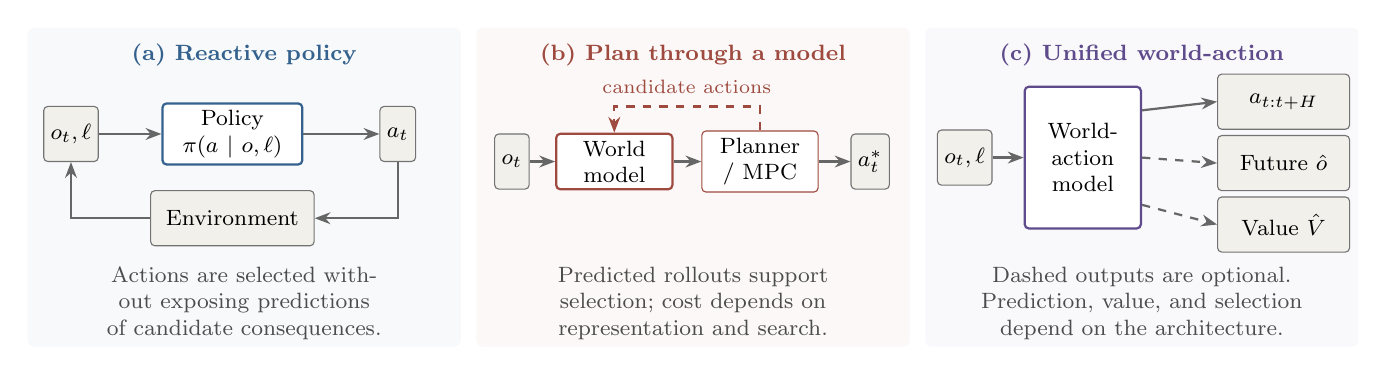
\begin{tikzpicture}[font=\figfont]
\tikzset{box/.style={fnode,inner sep=2.5pt,minimum height=7mm},
 caption/.style={align=center,text width=49mm,text=black!70,font=\figfont}}
\foreach \x/\c in {0/cVLA,5.7/cWM,11.4/cCONV}{
 \fill[\c!4,rounded corners=2pt] (\x,-2.35) rectangle +(5.5,4.05);}
\begin{scope}
\node[font=\figfont\bfseries,cVLA] at (2.75,1.35) {(a) Reactive policy};
\node[box,fill=cPale] (o) at (.55,.35) {$o_t,\ell$};
\node[box,draw=cVLA,thick,text width=16mm] (p) at (2.6,.35) {Policy\\$\pi(a\mid o,\ell)$};
\node[box,fill=cPale] (a) at (4.7,.35) {$a_t$};
\node[box,fill=cPale,text width=19mm] (e) at (2.6,-.72) {Environment};
\draw[farr] (o)--(p); \draw[farr] (p)--(a);
\draw[farr] (a.south)|-(e.east); \draw[farr] (e.west)-|(o.south);
\node[caption] at (2.75,-1.8) {Actions are selected without exposing predictions of candidate consequences.};
\end{scope}
\begin{scope}[xshift=5.7cm]
\node[font=\figfont\bfseries,cWM] at (2.75,1.35) {(b) Plan through a model};
\node[box,fill=cPale] (o) at (.45,0) {$o_t$};
\node[box,draw=cWM,thick,text width=13mm] (m) at (1.75,0) {World model};
\node[box,draw=cWM,text width=13mm] (p) at (3.6,0) {Planner / MPC};
\node[box,fill=cPale] (a) at (5,0) {$a_t^*$};
\draw[farr] (o)--(m); \draw[farr] (m)--(p); \draw[farr] (p)--(a);
\draw[farr,cWM,dashed] (p.north)--(3.6,.7)--(1.75,.7)--(m.north);
\node[inner sep=1.5pt,text=cWM,font=\fontsize{7.5}{9}\selectfont] at (2.67,.95) {candidate actions};
\node[caption] at (2.75,-1.8) {Predicted rollouts support selection; cost depends on representation and search.};
\end{scope}
\begin{scope}[xshift=11.4cm]
\node[font=\figfont\bfseries,cCONV] at (2.75,1.35) {(c) Unified world-action};
\node[box,fill=cPale] (o) at (.5,.05) {$o_t,\ell$};
\node[box,draw=cCONV,thick,text width=13mm,minimum height=18mm] (m) at (2,.05) {World-action model};
\node[box,fill=cPale,text width=15mm] (a) at (4.55,.76) {$a_{t:t+H}$};
\node[box,fill=cPale,text width=15mm] (s) at (4.55,-.02) {Future $\hat{o}$};
\node[box,fill=cPale,text width=15mm] (v) at (4.55,-.8) {Value $\hat{V}$};
\draw[farr] (o)--(m); \draw[farr] ([yshift=6mm]m.east)--(a.west);
\draw[farr,dashed] (m.east)--(s.west);
\draw[farr,dashed] ([yshift=-6mm]m.east)--(v.west);
\node[caption] at (2.75,-1.8) {Dashed outputs are optional. Prediction, value, and selection depend on the architecture.};
\end{scope}
\end{tikzpicture}
\end{document}
